\documentclass[conference]{IEEEtran}
\IEEEoverridecommandlockouts
\usepackage{cite}
\usepackage{amsmath,amssymb,amsfonts}
\usepackage{algorithmic}
\usepackage{graphicx}
\usepackage{textcomp}
\usepackage{xcolor}
\def\BibTeX{{\rm B\kern-.05em{\sc i\kern-.025em b}\kern-.08em
    T\kern-.1667em\lower.7ex\hbox{E}\kern-.125emX}}

%me
\usepackage[brazil]{babel}
\usepackage{bm}
\newcommand\w{1.0}

%para colocar a figura 6 no topo da pagina
\makeatletter
\setlength{\@fptop}{0pt}
\makeatother


\begin{document}

\title{ELE075 - Sistemas Nebulosos\\ Atividade Prática 2 - Parte 1
}

\author{\IEEEauthorblockN{ Gabriel Lara \\
José Geraldo Fernandes}
\IEEEauthorblockA{Escola de Engenharia \\
Universidade Federal de Minas Gerais \\
Belo Horizonte, Brasil}
}

\maketitle

% overleaf:
% https://www.overleaf.com/1962355144hnmknycbhfhg

\section{}  %num1

\[
Q = 
\begin{vmatrix}
0 & 0.8 & 0.6 & 0.25 \\
0.7 & 0.98 & 0.15 & 0.5 \\
\end{vmatrix}
\]

\[
R = 
\begin{vmatrix}
1 & 0.4 & 0.2 \\
0.1 & 0.4 & 0.7 \\
0.4 & 0.15 & 0.05 \\
0.85 & 0.3 & 0.1 \\
\end{vmatrix}
\]

\[
L = 
\begin{vmatrix}
1 & 0.2 & 0.6 & 0.8 \\
0.85 & 0.3 & 0.8 & 0.88 \\
\end{vmatrix}
\]

\hfill


\hspace{1cm}

\[
M = Q \wedge \neg L = 
\begin{vmatrix}
m_{11} & m_{12} & m_{13} & m_{14} \\
m_{21} & m_{22} & m_{23} & m_{24} \\
\end{vmatrix}
\]

\hspace{1cm}

em que $m_{ij} = min(Q_{ij}, 1 - L_{ij})$

\hspace{1cm}

$m_{11} = min(0, 0) = 0$

$m_{12} = min(0.8, 0.8) = 0.8$

$m_{13} = min(0.6, 0.4) = 0.4$

$m_{14} = min(0.25, 0.2) = 0.2$

\hspace{1cm}

$m_{21} = min(0.7, 0.15) = 0.15$

$m_{22} = min(0.98, 0.7) = 0.7$

$m_{23} = min(0.15, 0.2) = 0.15$

$m_{24} = min(0.5, 0.12) = 0.12$


\[
M = Q \wedge \neg L = 
\begin{vmatrix}
0 & 0.8 & 0.4 & 0.2 \\
0.15 & 0.7 & 0.15 & 0.12 \\
\end{vmatrix}
\]


\hspace{1cm} 


\[
P = Q \circ R = 
\begin{vmatrix}
p_{11} & p_{12} & p_{13} \\
p_{21} & p_{22} & p_{23} \\
\end{vmatrix}
\]

\hspace{1cm}

em que $p_{ij} = max(Q_{i,*} * R_{*, j})$ com a
operação $*$ representando multiplicação par a par.

\hspace{1cm}

$p_{11} = max((1, 0.1, 0.4, 0.85) * (0, 0.8, 0.6, 0.25))$

$p_{11} = max(0, 0.081, 0.24, 0.2125)$

$p_{11} = 0.24$

\hspace{.5cm}

$p_{12} = max((0.4, 0.4, 0.15, 0.3) * (0, 0.8, 0.6, 0.25))$

$p_{12} = max(0, 0.32, 0.09, 0.075)$

$p_{12} = 0.32$

\hspace{.5cm}

$p_{13} = max((0.2, 0.7, 0.05, 0.1) * (0, 0.8, 0.6, 0.25))$

$p_{13} = max(0, 0.56, 0.03, 0.025)$

$p_{13} = 0.56$

\hspace{.5cm}

$p_{21} = max((0.1, 0.1, 0.4, 0.85) * (0.7, 0.98, 0.15, 0.5)$

$p_{21} = max(0.7, 0.098, 0.06, 0.425)$

$p_{21} = 0.7$

\hspace{.5cm}

$p_{22} = max((0.4, 0.4, 0.15 0.3) * (0.7, 0.98, 0.15, 0.5)$

$p_{22} = max(0.28, 0.392, 0.0225, 0.15)$

$p_{22} = 0.392$

\hspace{.5cm}

$p_{23} = max((0.2, 0.7, 0.05, 0.1) * (0.7, 0.98, 0.15, 0.5)$

$p_{23} = max(0.14, 0.686, 0.0075, 0.05)$

$p_{23} = 0.686$

\[
P = Q \circ R = 
\begin{vmatrix}
0.24 & 0.32 & 0.56 \\
0.7 & 0.392 & 0.686 \\
\end{vmatrix}
\]

\hfill
\section{}  %num2

\[
A = 
\begin{vmatrix}
1 & 0.5 & 0.4 & 0.2 \\
\end{vmatrix}
\]

\[
R = 
\begin{vmatrix}
1 & 0.8 & 0 & 0 \\
0.8 & 1 & 0.8 & 0 \\
0 & 0.8 & 1 & 0.8 \\
0 & 0 & 0.8 & 1 \\
\end{vmatrix}
\]

\hfill
\[
B = A \circ R = 
\begin{vmatrix}
b1 & b2 & b3 & b4 \\
\end{vmatrix}
\]

em que $b_{i} = max(min(A_{i}, R_{*, i}))$

\hspace{.5cm}

$b_1 = max(min((1, 0.5, 0.4, 0.2), (1, 0.8, 0, 0))$

$b_1 = max(1, 0.5, 0, 0)  = 1 $

\hspace{.5cm}
 
$b_2 = max(min((1, 0.5, 0.4, 0.2), (0.8, 1, 0.8, 0))$

$b_2 = max(0.8, 0.5, 0.4, 0) = 0.8$ 

\hspace{.5cm}

$b_3 = max(min((1, 0.5, 0.4, 0.2), (0, 0.8, 1, 0.8))$

$b_3 = max(0, 0.5, 0.4, 0.2) = 0.5$

\hspace{.5cm}

$b_4 = max(min((1, 0.5, 0.4, 0.2), (0, 0, 0.8, 1))$

$b_4 = max(0, 0, 0.4, 0.2) = 0.4$

\hspace{1cm}

\[
B = A \circ R = 
\begin{vmatrix}
1 & 0.8 & 0.5 & 0.4 \\
\end{vmatrix}
\]

\hfill
\section{}  %num3

\par As curvas de pertinências são como na Figura \ref{fig:plot03}.

\[\mu_{young}(x) = gaussian(x, 0, 20)\]
\[\mu_{old}(x) = gaussian(x, 100, 30)\]

\begin{figure}[htbp]
\centering
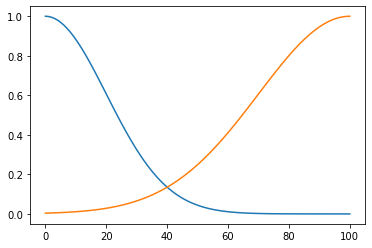
\includegraphics[width=\w\linewidth]{fig/plot03.png}
\caption{Curvas de pertinência, em azul $\mu_{young}$ e em laranja $\mu_{old}$}
\label{fig:plot03}
\end{figure}

\hfill
\section{}  %num4

\par As curvas de pertinências são como na Figura \ref{fig:plot04}.

\[\mu_{a}(x) = \neg \mu_{young}^2 \wedge \neg \mu_{old}^2\]
\[\mu_{b}(x) = \mu_{young}^2 \wedge \mu_{old}^2\]

\begin{figure}[htbp]
\centering
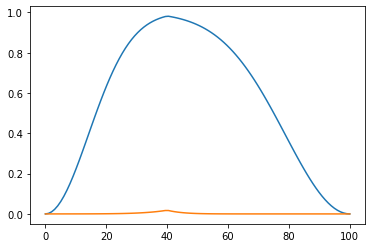
\includegraphics[width=\w\linewidth]{fig/plot04.png}
\caption{Curvas de pertinência, em azul $\mu_{a}$ e em laranja $\mu_{b}$}
\label{fig:plot04}
\end{figure}

\hfill
\section{}  %num5

\[
A_1 = 
\begin{vmatrix}
0.2 & 0.4 & 0.5 \\
\end{vmatrix}
\]

\[
A_2 = 
\begin{vmatrix}
1 & 1 & 0.3 \\
\end{vmatrix}
\]

\[
B_1 = 
\begin{vmatrix}
0.1 & 0.3 \\
\end{vmatrix}
\]

\[
B_1 = 
\begin{vmatrix}
0.6 & 0.2 \\
\end{vmatrix}
\]

\[A_1 \rightarrow B_1\]
\[A_2 \rightarrow B_2\]

\[
A' = 
\begin{vmatrix}
0 & 1 & 0 \\
\end{vmatrix}
\]

\hfill

%solucao por w

\[
\mu_{B'} = \underset{i}{\vee} [\vee (\mu_{A'} \wedge \mu_{A_i}) \wedge \mu_{B_i}]
\]

\[i = 1\]

\[
\mu_{B'_1} = \vee (\mu_{A'} \wedge \mu_{A_1}) \wedge \mu_{B_1} = \omega_1 \wedge \mu_{B_1}
\]

%min(0, 0.2), min(1, 0.4) e min(0, 0.5)
%aqui acho q o correto seria mu = 0/x1 + 0.4/x2 + 0/x3, mas essa anotaçao é mais chata(?)
\[
\mu_{B'_1} = \vee (
\begin{vmatrix}
0 & 0.4 & 0 \\
\end{vmatrix}
) \wedge \mu_{B_1} = 0.4 \wedge \mu_{B_1}
\]

%min(0.4, 0.1) e min(0.4, 0.3)
\[
\mu_{B'_1} = 
\begin{vmatrix}
0.1 & 0.3 \\
\end{vmatrix}
\]


\[i = 2\]

\[
\mu_{B'_2} = \vee (\mu_{A'} \wedge \mu_{A_2}) \wedge \mu_{B_2} = \omega_2 \wedge \mu_{B_2}
\]

%min(0, 1), min(1, 1) e min(0, 0.3)
\[
\mu_{B'_2} = \vee (
\begin{vmatrix}
0 & 1 & 0 \\
\end{vmatrix}
) \wedge \mu_{B_1} = 1 \wedge \mu_{B_2}
\]

%min(1, 0.6) e min(1, 0.2)
\[
\mu_{B'_1} = 
\begin{vmatrix}
0.6 & 0.2 \\
\end{vmatrix}
\]

\[
\mu_{B'} = \mu_{B'_1} \vee \mu_{B'_2} = 
\begin{vmatrix}
0.6 & 0.3 \\
\end{vmatrix}
= 0.6/y_1 + 0.3/y_2
\]

\hfill
\section{}  %num6

\par A curva de pertinência é como na Figura \ref{fig:plot06}.

\[
\mu_{A_1} = trapmf(x, 
\begin{bmatrix}
3 & 4 & 5 & 6 \\
\end{bmatrix})
\]

\[
\mu_{A_2} = trapmf(x, 
\begin{bmatrix}
6 & 6.5 & 7 & 7.5 \\
\end{bmatrix})
\]

\[
\mu_{C_1} = trimf(x, 
\begin{bmatrix}
3 & 4 & 5 \\
\end{bmatrix})
\]

\[
\mu_{C_2} = trimf(x, 
\begin{bmatrix}
4 & 5 & 6 \\
\end{bmatrix})
\]

\[A_1 \rightarrow C_1\]
\[A_2 \rightarrow C_2\]

\[
\mu_{A'} = trimf(x, 
\begin{bmatrix}
5 & 6 & 7 \\
\end{bmatrix})
\]

\hfill

%mt confuso?
\[
\mu_{C'} = \underset{i}{\vee} [\vee (\mu_{A'} \wedge \mu_{A_i}) \wedge \mu_{C_i}]
\]

%\begin{figure}[t!] eu coloquei a figura no topo pq antes só tinha ela na coluna, ai ficava no meio do espaço em branco
\begin{figure}[htbp]
\centering
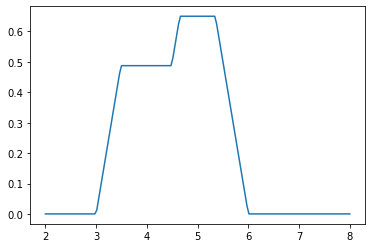
\includegraphics[width=\w\linewidth]{fig/plot06.png}
\caption{Curvas de pertinência de $C'$.}
\label{fig:plot06}
\end{figure}

\end{document}